%-----------------------------------------------
% Dateiname: Protype.tex
% Autor    : Stefano Kowalke <blueduck@gmx.net>
% Lizenz   : BSD
%-----------------------------------------------
\chapter{Prototypischer Nachweis der Herstellbarkeit}
\label{ch:protoype}

\begin{figure}[H]
    \centering
    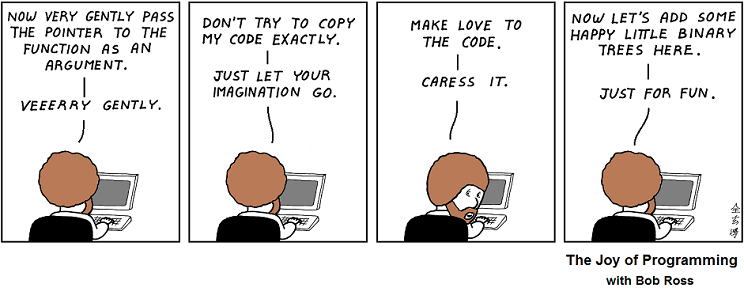
\includegraphics[scale=0.65]{gfx/the_art_of_happy_programming.png}
    \label{fig:bobRoss}
\end{figure}

Die Erstellung des Prototyps begann mit der Definition verschiedener Zielstellungen. Diese wurden in zusammenhängenden Arbeitspaketen zusammengefasst und dienten als Meileinsteine.

%-----------------------------------------------
% Dateiname: Concept.tex
% Autor    : Stefano Kowalke <blueduck@gmx.net>
% Lizenz   : BSD
%-----------------------------------------------
\section{Konzeption des Prototypen}
\label{prototype:sec:concept}
Bevor mit der Implementierung des Prototyps begonnen werden konnte, wurden die zu erreichenden Ziele definiert.

\begin{itemize}
\item Der Prototyp erhält den Extensionkey \textit{doctrine\_dbal}.
\item  Der Prototyp ist eine normale Extension, die über das \textit{Install Tool} installierbar ist. Dies ist notwendig, da bereits bei der Installation das zu nutzende \gls{dbms} auswählbar sein muß. Er ist gegenfalls ohne größeren Aufwand in eine Systemextension umwandelbar.
\item Der Prototyp unterstützt die alte Datenbank \gls{api}, damit TYPO3 CMS und externe Extensions weiterhin funktionieren.
\item Der Prototyp unterstützt MySQL als \gls{dbms}.
\item Die Methodennamen der neuen \gls{api} folgen den TYPO3 \gls{cgl}.
\item Die Erstellung der Basisdatenbank erfolgt durch Doctrine DBAL und nutzt dessen abstaktes Datenbankschema.
\item Der Prototyp nutzt intern \textit{Prepared Statements}.
\item Der Prototyp führt eine \textit{Fluent Query Language} ein, damit auf die manuelle Formulierung von SQL Anfragen verzichtet werden kann.
\end{itemize}

Diese Anforderungen konnten anschließend in einzelne Teilaufgaben zusammengefasst werden:

\begin{enumerate}
\item Erhöhung der Testabdeckung der vorhandenen Datenbank \gls{api}
\item Erstellen der Grundstrukutur des Prototypen
\item Integration in das \phpinline{Install Tool}
\item Implementation einer Fluent \gls{api}
\item Umbau von TYPO3 CMS auf die \gls{api} des Prototypen
\end{enumerate}

%-----------------------------------------------
% Dateiname: InstallTYPO3.tex
% Autor    : Stefano Kowalke <blueduck@gmx.net>
% Lizenz   : BSD
%-----------------------------------------------
\section{Installation von TYPO3 CMS}
\label{prototype:sec:installTYPO3}
\subsection{Verzeichnisse}
Zuerst wurde das Verzeichnis \pdf{thesis.dev/http} angelegt, welches als Wurzelverzeichnis der Installation über den Browser über die \textit{URL} erreichbar ist.

\begin{Verbatim}[samepage=true]
$ cd Sites/
$ mkdir -p thesis.dev/http/
$ cd thesis.dev/
\end{Verbatim}


Damit auf den Quellcode von TYPO3 CMS nicht über den Browser zugegriffen werden kann, wurde es per GIT nach \pdf{thesis.dev/typocms} heruntergeladen. Danach wurde nach \pdf{http} gewechselt und die notwendigen Symlinks und Verzeichnisse angelegt. Listing~\ref{lst:thesisDevFolders} zeigt die so erstellte Verzeichnisstruktur:

\begin{Verbatim}[samepage=true]
$ tree -L 2 --dirsfirst
.
├── http
│   ├── fileadmin
│   ├── typo3 -> typo3_src/typo3
│   ├── typo3_src -> ../typo3cms
│   ├── typo3conf
│   ├── uploads
│   └── index.php -> typo3_src/index.php
└── typo3cms
├── typo3
├── ChangeLog
├── GPL.txt
├── INSTALL.md
├── LICENSE.txt
├── NEWS.md
├── README.md
├── _.htaccess
├── composer.json
└── index.php
\end{Verbatim}

Danach wurde in der Hostdatei mittels \shinline{sudo sh -c "echo '127.0.0.1 thesis.dev' >> /etc/hosts"} ein A-Record der Domain \url{thesis.dev} angelegt und anschließend ein virtueller Host in der Apache2 Konfiguration erstellt, der auf das Verzeichnis \pdf{thesis.dev/http} zeigt.

\begin{shcode}
<VirtualHost *:80>¬
DocumentRoot "~/Sites/thesis.dev/http"¬
ServerName thesis.dev¬
ErrorLog "~/Sites/thesis.dev/logs/error_log"¬
CustomLog "~/Sites/thesis.dev/logs/access_log" common¬
</VirtualHost>
\end{shcode}

Im Anschluß daran wurde eine leere Datenbank mit dem Namen \texttt{thesis} erstellt:

\begin{shcode}
mysql -u root -p
MariaDB [(none)]> create database if not exists thesis;
Query OK, 1 row affected (0.01 sec)
	MariaDB [(none)]> quit;
	\end{shcode}

	Durch das Aufrufen von \url{http://thesis.dev/} im Browser wird der Installationsprozess gestartet, der in fünf Schritten das System installiert.

	\subsection{Schritt 1 - Systemcheck}
	Im ersten Schritt (Abb.:~\ref{fig:installTYPO3LegacyStepOne}) prüft das \textit{Install Tool} ob alle Verzeichnisse und Symlinks angelegt wurden und die entsprechenden Benutzerrechte besitzen. Intern werden hier Verzeichnisse wie \pdf{typo3temp} und Dateien wie \pdf{LocalConfiguration} angelegt. 

	\subsection{Schritt 2 - Eingabe der Datenbankdaten}
	Im zweiten Schritt (Abb.:~\ref{fig:installTYPO3LegacyStepTwo})werden die Benutzerdaten für die Datenbank eingegeben. Es kann hier zwischen einer Port- oder Socket-basierten Verbindung ausgewählt werden.

	Über den Button am Ende der Formulars wird – anstelle der nativen Datenbank API – die Systemextension DBAL genutzt, da TYPO3 CMS ein anderes \gls{dbms} nutzen soll. Die Exension wird daraufhin installiert und in ähnlicher Weise konfiguriert, wie es hier dargestellt wird. 

	\subsection{Schritt 3 - Auswahl der Datenbank}
	Nachdem die Verbindungsdaten eingegeben wurden, versucht TYPO3 CMS sich mit dem \gls{dbms} zu verbinden. Gelingt dies, werden alle verfügbaren Datenbanken abgefragt und aufgelistet (Abb.:~\ref{fig:installTYPO3LegacyStepThree}). Über die Auswahl kann eine leere Datenbank festgelegt beziehungsweise kann über das Inputfeld eine zu erstellende Datenbank angegeben werden. Durch die Aktivierung der Schaltfläche werden die Basistabellen in der Datenbank angelegt.

	\subsection{Schritt 4 - Einrichten eines TYPO3 Administrators}
	In 4. Schritt (Abb.:~\ref{fig:installTYPO3LegacyStepFour}) der Installation wird ein Administrator für die Seite eingerichtet und es kann ein Name für die Seite vergeben werden.

	\subsection{Schritt 5 - Abschluß der Installation}
	Danach ist die Installation abgeschlossen und über die Schaltfläche kann das Backend aufgerufen werden (Abb.:~\ref{fig:installTYPO3LegacyStepFive})

	\begin{figure}[H]
		\begin{subfigure}[b]{0.5\textwidth}
			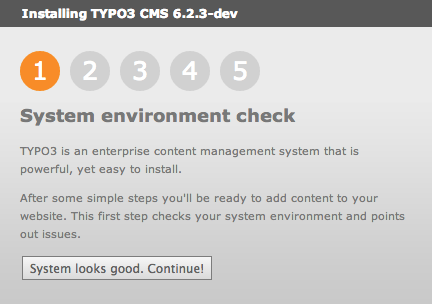
\includegraphics[width=\textwidth]{InstallingTYPO3/DoctrineDBAL/01-SystemEnvironmentCheck.png}
			\caption{Installation TYPO3 CMS - 1. Schritt}
			\label{fig:installTYPO3LegacyStepOne}
		\end{subfigure}%
		~ %add desired spacing between images, e. g. ~, \quad, \qquad, \hfill etc.
	%(or a blank line to force the subfigure onto a new line)
		\begin{subfigure}[b]{0.5\textwidth}
			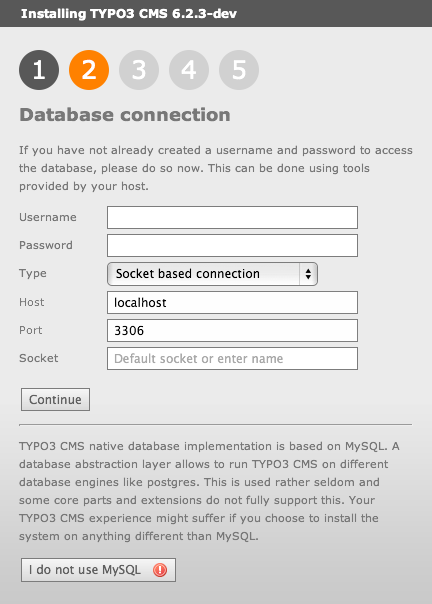
\includegraphics[width=\textwidth]{InstallingTYPO3/Legacy/02-DatabaseConnectionLegacy.png}
			\caption{Installation TYPO3 CMS - 2. Schritt}
			\label{fig:installTYPO3LegacyStepTwo}
		\end{subfigure}
		~ %add desired spacing between images, e. g. ~, \quad, \qquad, \hfill etc.
	%(or a blank line to force the subfigure onto a new line)
		\begin{subfigure}[b]{0.5\textwidth}
			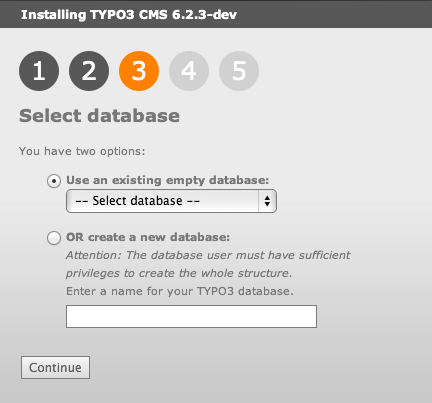
\includegraphics[width=\textwidth]{InstallingTYPO3/Legacy/03-SelectDatabaseLegacy.png}
			\caption{Installation TYPO3 CMS - 3. Schritt}
			\label{fig:installTYPO3LegacyStepThree}
		\end{subfigure}%
		~ %add desired spacing between images, e. g. ~, \quad, \qquad, \hfill etc.
	%(or a blank line to force the subfigure onto a new line)
		\begin{subfigure}[b]{0.5\textwidth}
			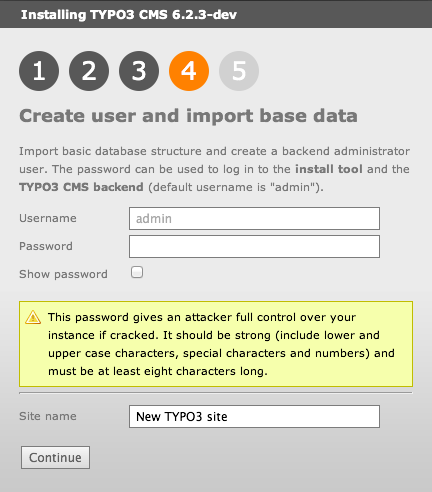
\includegraphics[width=\textwidth]{InstallingTYPO3/Legacy/04-CreateUserAndImportBaseDataLegacy.png}
			\caption{Installation TYPO3 CMS - 4. Schritt}
			\label{fig:installTYPO3LegacyStepFour}
		\end{subfigure}
		~ %add desired spacing between images, e. g. ~, \quad, \qquad, \hfill etc.
	%(or a blank line to force the subfigure onto a new line)
		\begin{subfigure}[b]{0.5\textwidth}
			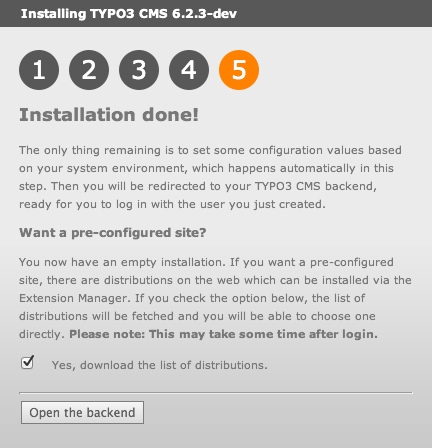
\includegraphics[width=\textwidth]{InstallingTYPO3/Legacy/05-InstallationDoneLegacy.png}
			\caption{Installation TYPO3 CMS - 5. Schritt}
			\label{fig:installTYPO3LegacyStepFive}
		\end{subfigure}%
		\caption{Installation von TYPO3 CMS}
		\label{fig:installationOfTYPO3}
	\end{figure}

%-----------------------------------------------
% Dateiname: CreateTestsForOldAPI.tex
% Autor    : Stefano Kowalke <blueduck@gmx.net>
% Lizenz   : BSD
%-----------------------------------------------
\section{Implementation von Unit Tests der alten Datenbank API}
\label{prototype:sec:createTestForOldAPI}
Um zu gewährleisten, dass TYPO3 CMS sowohl mit der alten API - die von dem Prototypen zur Verfügung gesellt wird - als auch mit der neuen API kompatibel ist, müssen Untit Tests für die alte Datenbank API geschrieben werden. 

Zur Ausführung der Unit Tests wird die Extension \textit{PHPUnit} benötigt, welche das gleichnamige Testing Framework \textit{PHPUnit\footnote{\url{http://www.phpunit.de}}} zur Verfügung und einen einen graphischen Testrunner im Backend mitbringt. Sie wird über den Extension Manager installiert.

Die alte Datenbank API verfügt zur dem Zeitpunkt der Erstelltung des Prototypen über 40 Tests mit 49 Assertions, welche jedoch lediglich Hilfsmethoden testen. Im Laufe der Arbeit wurden wurden 68 Tests implementiert, die alle Methoden testen. Die Abbildung~\ref{fig:executeUnitTestsForOldAPI} zeigt die Ausführung der von TYPO3 CMS mitgelieferten Unit Tests; Abbildung~\ref{fig:executeNewUnitTestsForOldAPI} zeigt die Ausführung der neu implementierten sowie der alten Tests.

\begin{figure}[H]
    \centering
    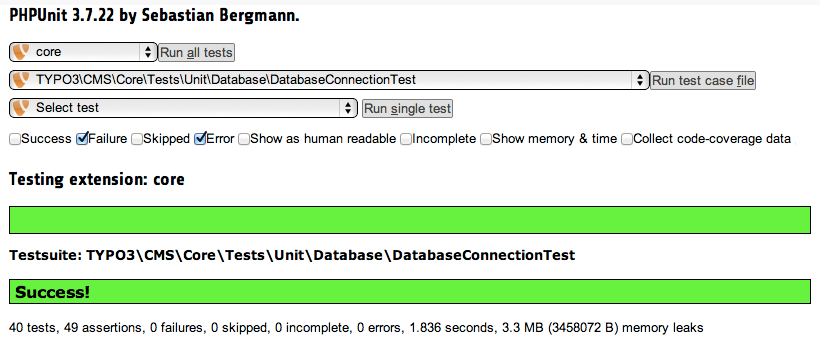
\includegraphics[scale=0.5]{TYPO3/DatabaseConnectionUnitTestsLegacy.png}
    \caption{Ausführung der vorhandenen Unit Tests für die alte Datenbank API}
    \label{fig:executeUnitTestsForOldAPI}
\end{figure}

\begin{figure}[H]
    \centering
    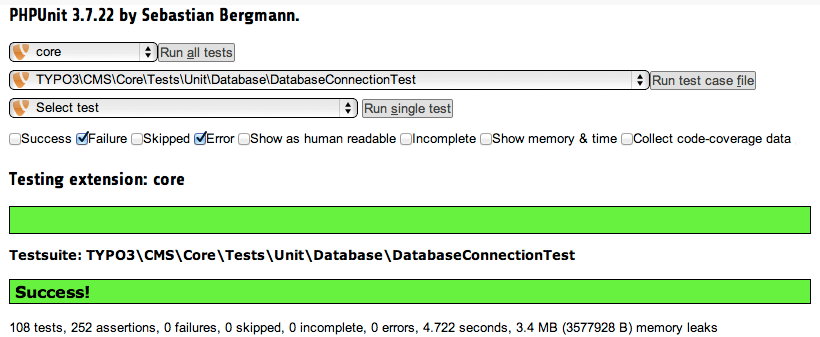
\includegraphics[scale=0.5]{TYPO3/DatabaseConnectionAddedUnitTestsLegacy.png}
    \caption{Ausführung der vorhandenen und hinzugefügten Unit Tests für die alte Datenbank API}
    \label{fig:executeNewUnitTestsForOldAPI}
\end{figure}

%-----------------------------------------------
% Dateiname: CreatePrototype.tex
% Autor    : Stefano Kowalke <blueduck@gmx.net>
% Lizenz   : BSD
%-----------------------------------------------
\section{Erstellung des Prototypen}
\label{prototype:sec:createPrototype}

Die Grundstruktur der Extension wurde unter \pdf{thesis/http/typo3conf/ext/doctrine\_dbal} erstellt.

\begin{Verbatim}[samepage=true]
thesis.dev/http/typo3con/ext/
├── doctrine_dbal/
│   ├── Configuration/
│   ├── Resources/
│   ├── ext_emconf.php
│   ├── ext_icon.gif
│   └── ext_tables.php
\end{Verbatim}

Die Datei \pdf{ext\_emconf.php} enthält die Metainformationen der Extension, die von dem Extension Manager verarbeitet werden.

\begin{listing}
\begin{phpcode}
<?php
$EM_CONF[$_EXTKEY] = array(
	'title' => 'Doctrine DBAL',
	'description' => 'Doctrine DBAL Integration in TYPO3 CMS',
	'category' => 'be',
	'author' => 'Stefano Kowalke',
	'author_email' => 'blueduck@gmx.net',
	'author_company' => 'Skyfillers GmbH',
	'shy' => 0,
	'priority' => '',
	'module' => 'mod1',
	'state' => 'alpha',
	'internal' => 0,
	'uploadfolder' => 0,
	'createDirs' => '',
	'modify_tables' => '',
	'clearCacheOnLoad' => 0,
	'lockType' => '',
	'version' => '0.1.0',
	'constraints' => array(
		'depends' => array(
			'typo3' => '6.2.0-6.2.99',
		),
		'conflicts' => array('adodb', 'dbal'),
		'suggests' => array(
		),
	),
);
\end{phpcode}
\caption{Die Datei ext\_emconf.php}
\label{lst:extEmconf}
\end{listing}

Danach wurden die Datei \pdf{DatabaseConnection.php} von TYPO3 CMS in den Ordner \pdf{Classes/Persistence/Legacy} des Prototypen kopiert.

Damit TYPO3 CMS diese Dateien anstelle der Originalen verwendet, wurde diese per XCLASS in der Datei \pdf{ext\_localconf.php} registiert.

\begin{listing}[H]
\begin{phpcode}
if (!defined('TYPO3_MODE')) {
	die('Access denied.');
}

$GLOBALS['TYPO3_CONF_VARS']['SYS']['Objects']['TYPO3\\CMS\\Core\\Database\\DatabaseConnection'] =
  array('className' => 'Konafets\\DoctrineDbal\\Persistence\\Legacy\\DatabaseConnection');
\end{phpcode}
\caption{Registrierung der XCLASSes in \pdf{doctrine\_dbal/ext\_localconf.php}}
\label{lst:xclassDatabaseAPI}
\end{listing}

Zur Überprüfung ob TYPO3 CMS tatsächlich diese Klasse nutzt, wurde der Prototyp über den Extension Manager installiert und in der \gls{ide} ein Debug-Breakpoint in die Klasse\\ \phpinline{Konafets\DoctrineDbal\Persistence\Legacy\DatabaseConnection} innerhalb der \phpinline{connectDB} gesetzt, an dem die \gls{ide} die Ausfühung von TYPO3 CMS anhält, wenn dieser erreicht wird.

Die \gls{ide} verfügt über einen Debug Listener, der auf ein vom Browser gesendetes Token wartet und bei Empfang den Debug Prozess startet. Für den verwendeten Browser \textit{Chrome} ist ein Addon verfügbar, mittels diesem das Senden des Debug-Tokens per Knopfdruck ein- und ausgeschaltet werden kann.

Wird der Browser und die \gls{ide} in den Debug-Modus gesetzt und TYPO3 CMS neugeladen, bleibt das Programm an dem gesetzten Breakpoint stehen.

Die Klasse, die die neue API beherbergen wird, wurde in unter\\ \pdf{doctrine\_dbal/Classes/Persistence/Doctrine} mit dem Namen \pdf{DatabaseConnection.php} erstellt. Da die alte API vorerst nicht verändert werden soll, denoch die Methoden der neuen API definiert und getestet werden sollen, erbt die Klasse\\ \phpinline{\Konafets\DoctrineDbal\Persistence\Doctrine\DatabaseConnection} von der alten Klasse \phpinline{\Konafets\DoctrineDbal\Persistence\Legacy\DatabaseConnection}.
Intern rufen sie die Methoden der Elternklasse auf.

\begin{figure}[H]
    \centering
    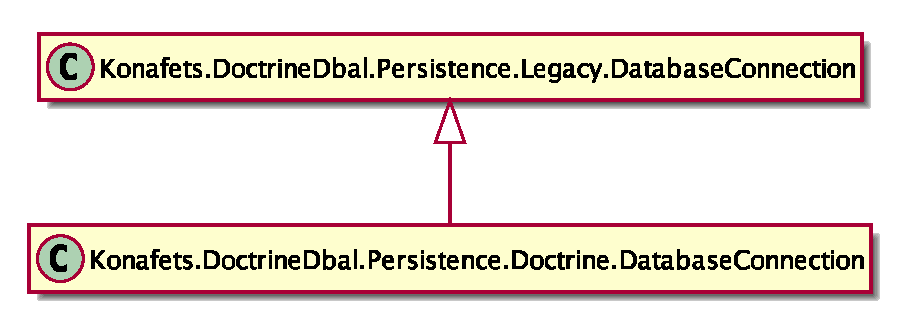
\includegraphics[scale=0.5]{gfx/uml/NewAPI/DatabaseConnectionExtentsFromOldAPI.eps}
    \caption{Neue API-Klasse erbt von alter API-Klasse}
    \label{fig:newDatabaseConnectionExtendsFromOldOne}
\end{figure}

\begin{phpcode}
class DatabaseConnection extends
\Konafets\DoctrineDbal\Persistence\Legacy\DatabaseConnection {
    /**
	 * Select a SQL database
	 *
	 * @return boolean Returns TRUE on success or FALSE on failure.
	 */
	public function selectDatabase() {
		return parent::sql_select_db();
	}

	/**
	 * Connects to database for TYPO3 sites:
	 *
	 * @throws \RuntimeException
	 * @throws \UnexpectedValueException
	 *
	 * @return void
	 * @api
	 */
	public function connectDatabase() {
		parent::connectDB();
	}
\end{phpcode}

Parallel dazu wurden die Unit Tests der alten API nach \pdf{doctrine\_dbal/Tests/Persistence/Legacy/} kopiert und an die neue API angepasst. Da die Anfragen an die neue API zu diesem Zeitpunkt von ihr lediglich an die alte API delegiert werden, funktionieren die Unit Tests weiterhin.

Die letzte Aufgabe des ersten Meilensteins bestand aus dem Refactoring der Methode \phpinline{connectDB()}. Dabei wird der Code der Methode verändert ohne die Funktion zu veränderen. Refactorings werden durchgeführt, um den Code zu vereinfachen.

Anhand des Methodennamen ist zu erkennen, dass sie für die Etablierung einer Verbindung zur Datenbank zuständig ist, tatsächlich unterschiedliche Aufgaben selbst implementiert. So hat sie:

\begin{itemize}
	\item einen Test durchgeführt, ob eine Datenbank konfiguriert ist
	\item die Verbindung angefordert
	\item die konfigurierte Datenbank ausgewählt und
	\item verschiedene Hooks ausgeführt
\end{itemize}

Das folgende Listing zeigt die Methode vor dem Refactoring.

\begin{phpcode}
public function connectDB($host = NULL, $username = NULL, $password = NULL, $db = NULL) {
	// Early return if connected already
	if ($this->isConnected) {
		return;
	}

	if (!$this->databaseName && !$db) {
		throw new \RuntimeException(
			'TYPO3 Fatal Error: No database selected!',
			1270853882
		);
	}

	if ($host || $username || $password || $db) {
		$this->handleDeprecatedConnectArguments($host, $username, $password, $db);
	}

	if ($this->sql_pconnect()) {
		if (!$this->sql_select_db()) {
			throw new \RuntimeException(
				'TYPO3 Fatal Error: Cannot connect to the current database, "' .
				  $this->databaseName . '"!',
				1270853883
			);
		}
	} else {
		throw new \RuntimeException(
			'TYPO3 Fatal Error: The current username, password or host was not
			accepted when the connection to the database was attempted to be established!',
			1270853884
		);
	}

	// Prepare user defined objects (if any) for hooks which extend query methods
	$this->preProcessHookObjects = array();
	$this->postProcessHookObjects = array();
	if (is_array($GLOBALS['TYPO3_CONF_VARS']['SC_OPTIONS']['t3lib/class.t3lib_db.php']
				['queryProcessors'])) {
		foreach ($GLOBALS['TYPO3_CONF_VARS']['SC_OPTIONS']['t3lib/class.t3lib_db.php']
				['queryProcessors'] as $classRef) {
			$hookObject = GeneralUtility::getUserObj($classRef);
			if (!(
				$hookObject instanceof PreProcessQueryHookInterface
				|| $hookObject instanceof PostProcessQueryHookInterface
			)) {
				throw new \UnexpectedValueException(
					'$hookObject must either implement interface
					TYPO3\\CMS\\Core\\Database\\PreProcessQueryHookInterface or interface
					TYPO3\\CMS\\Core\\Database\\PostProcessQueryHookInterface',
					1299158548
				);
			}
			if ($hookObject instanceof PreProcessQueryHookInterface) {
				$this->preProcessHookObjects[] = $hookObject;
			}
			if ($hookObject instanceof PostProcessQueryHookInterface) {
				$this->postProcessHookObjects[] = $hookObject;
			}
		}
	}
}
\end{phpcode}

Das folgende Listing zeigt die Methode bereits unter neuen Namen nach dem Refactoring. Code, der nicht zur definierten Aufgabe der Methode gehörte, wurde in eigene Methoden ausgelagert. Die Methode zur Überprüfung der veralteten Parameter konnte gänzlich entfallen. Zudem wurden für alle Eigenschaften der Klasse \textit{Getter}-Methoden eingeführt, die intern genutzt werden.

\begin{phpcode}
public function connectDatabase() {
	// Early return if connected already
	if ($this->isConnected) {
		return;
	}

	$this->checkDatabasePreconditions();

	try {
		$this->link = $this->getConnection();
	} catch (\Exception $e) {
		echo $e->getMessage();
	}

	$this->isConnected = $this->checkConnectivity();
	if ($this->isConnected) {
		$this->initCommandsAfterConnect();
		$this->selectDatabase();
	}

	$this->prepareHooks();
}
\end{phpcode}

Die Funktion der Methode konnte erfolgreich überprüft werden, indem von der Kindklasse die Methode \phpinline{connectDB()} der Elternklasse überschrieben wurde und intern \phpinline{connectDatabase()} aufruft.

Zum Ende des ersten Meilensteins bestand der Prototyp aus den folgenden Verzeichnissen und Dateien.

\begin{Verbatim}[samepage=true]
doctrine_dbal
├── Classes
│   └── Persistence
│       ├── Doctrine
│       │   ├── DatabaseConnection.php
│       └── Legacy
│           └── DatabaseConnection.php
├── Tests
│   └── Unit
│       └── Persistence
│           └── Legacy
│                └── DatabaseConnectionTest.php
├── ext_emconf.php
├── ext_icon.gif
├── ext_localconf.php
└── ext_tables.php
\end{Verbatim}

\subsection{Prototype über das Install Tool installieren}
Für eine Datenbankabstraktionsschicht ist es wichtig, dass sie bereits während der Installation verfügbar ist um ein alternatives \gls{dbms} nutzen zu können. Demnach muß der Prototyp – analog zur Systemextension DBAL - über das Install Tool installierbar sein, was zu geringfügigen Anpassungen am Install Tool führt.

Wie bei der Installation von TYPO3 CMS zu sehen war, führt das Install Tool in fünf Schritten durch die Installation. Diese Schritte werden von Klassen zur Verfügung gestellt, die sich im Ordner \pdf{typo3/sysext/install/Classes/Controller/Action/Step} befinden. Sie werden über den StepController \pdf{typo3/sysext/install/Classes/Controller/Action/StepController} gesteuert. Dabei iteriert der Controller bei jedem Reload des Installtools über alle Schritte und prüft ob der jeweils aktuelle Schritt bereits ausgeführt wurde oder noch ausgeführt werden muß. Der Controller erkennt dies an Bedingungen, die von jedem Schritt definiert werden.
Sind alle Bedingungen erfüllt, findet ein Redirekt auf den nächsten Schritt statt.

Die Ausgabe der Schritte erfolgt über verschiedene HTML-Template Dateien, die in der TYPO3 eigenen Template-Sprache \textit{Fluid} verfasst sind. Das Install Tool setzt hier das \gls{mvc}-Pattern ein, um die Geschäftslogik von der Präsentation zu trennen.

Die HTML-Templates unterteilen sich in \textit{Layouts}, \textit{Templates} und \textit{Partials}, die in den jeweilig gleichnamigen Verzeichnissen in \pdf{typo3/sysext/install/Resources/Privat/} zu finden sind.

\begin{itemize}
	\item Ein Template beschreibt die grundlegende Struktur einer Seite. Typischerweise befindet sich darin der Seitenkopf und -fuß.
	\item Die Struktur einer einzelnen Seite wird von einem Template festgelegt.
	\item  Partials stellen wiederkehrende Elemente einer Seite dar. Sie können in Layout- und Templatedateien eingebunden werden. Die Schaltfläche \textit{I do not use MySQL} aus Abbildung~\ref{fig:installTYPO3LegacyStepTwo} im zweiten Schritt ist ein Beispiel eines Partials.

Dieser Schritt stellt zudem den Anfangspunkt der Anpassungen dar. Es wurden zwei Partials erstellt und in das Template des Schrittes eingebunden. Das erste Partial stellt eine Schaltfläche dar, über die der Prototyp installiert werden kann, während das zweite eine Schaltfläche zur Deinstallation bereitstellt. \textit{Fluid} entscheidet anhand der Bedingung \texttt{isDoctrineEnabled} welches der beiden Partials angezeigt wird.
\end{itemize}

\begin{htmlcode}
<p>
TYPO3 CMS native database implementation is based on mysql. This feature
installs Doctrine DBAL and its experimental at the moment.
Use it at your own risk and when you know what you are doing.
</p>

<form method="post">
	<f:render partial="Action/Common/HiddenFormFields" arguments="{_all}" />
	<input type="hidden" value="execute" name="install[set]" />
	<input type="hidden" value="1" name="install[values][loadDoctrine]" />
	<button type="submit">
		I want use Doctrine DBAL
		<span class="t3-install-form-button-icon-negative">&nbsp;</span>
	</button>
</form>
\end{htmlcode}

\begin{htmlcode}
<f:if condition="{isDoctrineEnabled}">
	<f:then>
		<f:render partial="Action/Step/DatabaseConnect/UnloadDoctrineDbal" arguments="{_all}" />
	</f:then>

	<f:else>
		<f:render partial="Action/Step/DatabaseConnect/ConnectDetails" arguments="{_all}" />
		<f:render partial="Action/Step/DatabaseConnect/LoadDoctrineDbal" arguments="{_all}" />
		<f:render partial="Action/Step/DatabaseConnect/LoadDbal" arguments="{_all}" />
	</f:else>
</f:if>
\end{htmlcode}

\begin{figure}[H]
    \centering
    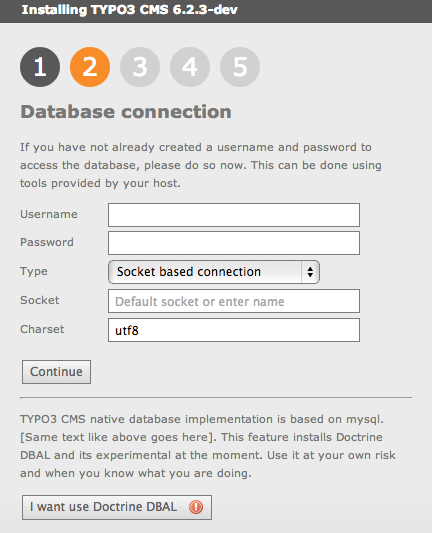
\includegraphics[scale=0.5]{InstallingTYPO3/DoctrineDBAL/02-DatabaseConnection.png}
    \caption{Hinzugefügte Schaltfläche um den Prototypen zu installieren}
    \label{fig:newDatabaseConnectionExtendsFromOldOne}
\end{figure}

Damit die Bedingung \texttt{isDoctrineEnabled} einen Wert enthält, muß diese von der Action des Schrittes definiert und an die View übergeben werden. In diesem Fall ist dafür die Klasse \phpinline{\TYPO3\CMS\Install\Controller\Action\Step\DatabaseConnect} zuständig. Hier wird der Extension Manager gefragt, ob der Prototyp installiert ist.

\begin{listing}
\begin{phpcode}
$isDbalEnabled =
  \TYPO3\CMS\Core\Utility\ExtensionManagementUtility::isLoaded('doctrine_dbal');

$this->view
  ->assign('isDoctrineEnabled', $isDoctrineEnabled)
  ->assign('username', $this->getConfiguredUsername())
  ->assign('password', $this->getConfiguredPassword())
  ->assign('host', $this->getConfiguredHost())
  ->assign('port', $this->getConfiguredOrDefaultPort())
  ->assign('database', $GLOBALS['TYPO3_CONF_VARS']['DB']['database'] ?: '')
  ->assign('socket', $GLOBALS['TYPO3_CONF_VARS']['DB']['socket'] ?: '');
\end{phpcode}
\caption{Zuweisung von in PHP definierten Variablen an die View}
\end{listing}

Durch den Klick auf die neu hinzugefügte Schaltfläche wird der Prototyp installiert. Dazu wird der per POST-Request gesendete Wert \texttt{loadDoctrine} von dem gleichen Schritt auswertet und per Extension Manager installiert (Siehe \pdf{typo3/sysext/install/Classes/Controller/Action/Step/DatabaseConnect.php} Zeilen 59-63 und 815-844). Daraufhin erhält der Benutzer ein visuelles Feedback, dass der Protoyp installiert wurde. Der weitere Verlauf der Installation ist mit der aus Kapitel~\ref{prototype:sec:installTYPO3} dargestellten Installation identisch.

\subsection{Umstellung auf Doctrine DBAL}
Nach den bisher vorgenommen Anpassungen ist der Prototyp zum Einen über das Install Tool, sowie über den Extension Manager im Backend installierbar. Anfragen an die Datenbank werden per XCLASS zum Prototypen geleitet. Dabei wird intern weiterhin die alte Datenbank API mit MySQLi genutzt.

Die nächste Aufgabe bestand darin den Prototypen auf Doctrine DBAL umzustellen, sowie das Install Tool daran anzupassen.

Um den Überblick zu behalten werden zunächst die Änderungen beschrieben, die am Prototypen notwendig wurden. Danach folgen die Anpassungen an TYPO3 CMS.

\subsubsection{Installation von Doctrine DBAL}
Doctrine DBAL wurde über \textit{Composer} installiert.

Composer ist ein Dependency Manager\footnote{https://getcomposer.org/} für PHP, welcher von der Kommandozeile aufgerufen wird. Es dient zum Auflösen von Abhängigkeiten eines Projektes. Diese Abhängigkeiten werden in einer \pdf{composer.json}-Datei definiert und durch Ausführung des Programms in Verbindung mit der Konfigurationsdatei in dem Ordner \pdf{vendor} installiert.

Für den Prototypen wurde Doctrine DBAL als externe Abhängigkeit in der \pdf{composer.json} wie folgt definiert:

\begin{listing}
\begin{jsoncode}
{
	"name": "typo3/doctrine_dbal",
	"type": "typo3-cms-extension",
	"description": "This brings Doctrine2 to TYPO3",
	"homepage": "http://typo3.org",
	"license": ["GPL-2.0+"],
	"version": "6.2.0",
	"require": {
		"doctrine/dbal": "dev-master"
	},
	"mininum-stability": "dev",
}
\end{jsoncode}
\caption{Die Datei composer.json}
\label{lst:composer}
\end{listing}

Durch das Kommando \shinline{composer install} erfolgt die Installation von Doctrine DBAL in den Ordner \pdf{vendor/doctrine}.

Composer Konfigurationsdateien werden seit TYPO3 CMS 6.2 analysiert. Aus den definierten Abhängigkeiten und den (System)-Extensions wird vom Package Mananger ein Graph von Abhängigkeiten aufgebaut welcher in \pdf{thesis.dev/http/typo3conf/PackagesStates.php} gespeichert wird. Diese Datei wird bei der Installation erstellt und stetig aktualisiert. Da diese Funktionalität relativ neu ist, mußte diese Datei bei der Installation des Prototypen manuell angepasst werden. Das wird später detailierter beschrieben.

Externe Abhängigkeiten werden vom Package Manager in \pdf{thesis.dev/http/Packages/Library} erwartet. Aus diesem Grund muß der Ordner \pdf{thesis.dev/http/typo3conf/ext/doctrine\_dbal/vendor/doctrine} nach \pdf{thesis.dev/http/Packages/Library/} kopiert werden.

Die Installation von Doctrine ist damit vorest abgeschlossen.

\subsubsection{Umstellung der neuen API auf Doctrine DBAL}
Die Integration von Doctrine DBAL sollte so transparent für TYPO3 CMS und die Extensions erfolgen, dass weiterhin über die Methoden der alten API auf die Datenbank zugegriffen werden konnte. Die alte API steht dabei vergleichbar einer Fassade vor der neuen API, die ankommende Anfragen selbst behandelt oder an die neue API delegiert. Dieses Vorgehen erlaubt die sukzessive Integration von Doctrine DBAL.

Um dies zu erreichen wurde die in Abbildung~\ref{fig:newDatabaseConnectionExtendsFromOldOne} vorgestellte Hierachie umgekehrt - die Klasse \phpinline{\Konafets\DoctrineDbal\Persistence\Legacy\DatbaseConnection} erbt nun von der neuen Klasse \phpinline{\Konafets\DoctrineDbal\Persistence\Doctrine\DatbaseConnection}.

![image](../gfx/uml/NewAPI/OldDatabaseConnectionExtentsFromNewAPI.png)

Anschließend wurde die Änderung der Klassenhierachie in \pdf{doctrine\_dbal/ext\_localconf.php}  bekannt gemacht.

\begin{phpcode}
$GLOBALS['TYPO3_CONF_VARS']['SYS']['Objects']['TYPO3\\CMS\\Core\\Database\\DatabaseConnection'] = array('className' => 'Konafets\\DoctrineDbal\\Persistence\\Legacy\\DatabaseConnection');
\end{phpcode}

Im nächsten Schritt wurden alle notwendigen Eigenschaften der alten Klasse in die neue Klasse verschoben. Jede Eigenschaft bekam zudem Setter- und Getter Methode, über die darauf zugegriffen werden soll.

\begin{phpcode}
	public function setDatabaseUsername($username) {
		$this->disconnectIfConnected();
		$this->connectionParams['user'] = $username;

		return $this;
	}

	public function getDatabaseUsername() {
		return $this->connectionParams['user'];
	}

	public function setStoreLastBuildQuery($value) {
		$this->store_lastBuiltQuery = (bool)$value;
	}
\end{phpcode}


Die Eigenschaften die die Konfigurationsinformation für die Datenbank bereithielten wurden entfernt und durch ein Konfigurationsarray ersetzt, welches Doctrine DBAL zum Anfordern einer Verbindung erwartet.

\begin{phpcode}
	protected $connectionParams = array(
		'dbname'   => '',
		'user'     => '',
		'password' => '',
		'host'     => 'localhost',
		'driver'   => 'pdo_mysql',
		'port'     => 3306,
		'charset'  => 'utf8',
	);
\end{phpcode}

Zum wurden verschiedene Doctrine-spezische Eigenschaften und Setter/Getter-Methoden der Klasse hinzugefügt.

Die eigentliche Umstellung auf Doctrine DBAL erfolgte in der Methode \phpinline{\Konafets\DoctrineDbal\Persistence\Doctrine\DatabaseConnection::getConnection()}, da sie das Verbindungsobjekt erstellt und zurückgibt.

Zunächst wurde Code, welcher nicht zum Aufgabengebiet der Methode gehört, in eigene Klassen ausgelagert. In dem Fall betraf das den Test nach einer installierten MySQLi PHP-Erweiterung, welcher im gleichen Zuge auf PDO geändert wurde.

Die Initialisierung von Doctrine erfolgt in einer eigenen Methode. Dort wird je eine Instanz von \phpinline{\Doctrine\DBAL\Configuration} und \phpinline{\Doctrine\DBAL\Schema\Schema}.

Die Methode der \phpinline{sql_pconnect()} der alten API bot die Möglichkeit einer persistenten Verbindung zur Datenbank. Dies wurde implementiert, in dem ein eigenes \phpinline{PDO}-Objekt mit dem Konstrukturparameter \phpinline{\PDO::ATTR_PERSISTENT => true} erstellt und in dem Konfigurationsarray gespeichert wurde.

Dieses Konfigurationsarray (siehe Listing~\ref{lst:DoctrineConfigArray}) wird \phpinline{\Doctrine\DBAL\DriverManager::getConnection()} übergeben, welches ein Verbindungsobjekt zurückgibt.

Zudem muß Doctrine DBAL der Datentyp \sqlinline{Enum} bekanntgemacht werden. Anschließend wird der Schema Manager erstellt, welcher zur Verwaltung des Datenbankschemas notwendig ist.

Am Schluß wird das Verbindungsobjekt zurückgegeben.

\begin{phpcode}
	/**
	 * Open a (persistent) connection to a MySQL server
	 *
	 * @return boolean|void
	 * @throws \RuntimeException
	 */
	public function getConnection() {
		if ($this->isConnected) {
			return $this->link;
		}

		$this->checkForDatabaseExtensionLoaded();

		$this->initDoctrine();

		// If the user want a persistent connection we have to create the PDO instance by ourself and pass it to Doctrine.
		// See http://stackoverflow.com/questions/16217426/is-it-possible-to-use-doctrine-with-persistent-pdo-connections
		// http://www.mysqlperformanceblog.com/2006/11/12/are-php-persistent-connections-evil/
		if ($this->persistentDatabaseConnection) {
			// pattern: mysql:host=localhost;dbname=databaseName
			$cdn = substr($this->getDatabaseDriver(), 3) . ':host=' . $this->getDatabaseHost() . ';dbname=' . $this->getDatabaseName();
			$pdoHandle = new \PDO($cdn, $this->getDatabaseUsername(), $this->getDatabasePassword(), array(\PDO::ATTR_PERSISTENT => true));
			$this->connectionParams['pdo'] = $pdoHandle;
		}

		$connection = DriverManager::getConnection($this->connectionParams, $this->databaseConfiguration);
		$this->platform = $connection->getDatabasePlatform();

		$connection->connect();

		// We need to map the enum type to string because Doctrine don't support it native
		// This is necessary when the installer loops through all tables of all databases it found using this connection
		// See https://github.com/barryvdh/laravel-ide-helper/issues/19
		$this->platform->registerDoctrineTypeMapping('enum', 'string');
		$this->schemaManager = $connection->getSchemaManager();

		return $connection;
	}
\end{phpcode}

Die Methode \phpinline{connectDatabase()} wurden dahingehen verändert, dass sie eine \phpinline{ConnectionException} wirft, wenn von \phpinline{getConnection()} keine Verbindung erstellt werden konnte. Die entsprechenden Exceptionklassen wurden in \pdf{doctrine\_dbal/Classes/Exeptions/} erstellt.

Die Methode \phpinline{query()} stellte in der alten API die zentrale Schnittstelle zum Senden der Anfragen an die Datenbank dar. Sie wird intern von allen Methoden verwendet um dessen SQL-Anfragen abzusenden. Intern nutzte sie die gleichnamige Methode von MySQLi. Die neue API übernimmt diese Funktionalität vollständig.

Wie bereits in Kapitel~\ref{sec:doctrine} erwähnt wurde, gibt \phpinline{query()} ein Statementobjekt zurück, welches die Ergebnismenge bereithält. Dort wurde ebenfalls dargestellt, dass diese Menge durch die Methode \phpinline{fetch()} in Verbindung mit PDO-Konstanten zum Beispiel in Index-basierte oder Assoziative Arrays formatiert werden kann.

Um die Arbeit mit der Ergebnismenge zu erleichtern wurden die drei Methoden \phpinline{fetchAssoc($stmt)}, \phpinline{fetchRow($stmt)} und \phpinline{$fetchColumn($stmt)} implementiert, die die am Häufigsten vorkommenden  \textit{Fetch-Styles} kapseln.

\begin{phpcode}
	/**
	 * Returns an associative array that corresponds to the fetched row, or FALSE if there are no more rows.
	 * Wrapper function for Statement::fetch(\PDO::FETCH_ASSOC)
	 *
	 * @param \Doctrine\DBAL\Driver\Statement $stmt A PDOStatement object
	 *
	 * @return boolean|array Associative array of result row.
	 * @api
	 */
	public function fetchAssoc($stmt) {
		if ($this->debugCheckRecordset($stmt)) {
			return $stmt->fetch(\PDO::FETCH_ASSOC);
		} else {
			return FALSE;
		}
	}

		public function fetchColumn($stmt, $index = 0) {
		if ($this->debugCheckRecordset($stmt)) {
			return $stmt->fetchColumn($index);
		} else {
			return FALSE;
		}
	}

		public function fetchRow($stmt) {
		if ($this->debugCheckRecordset($stmt)) {
			return $stmt->fetch(\PDO::FETCH_NUM);
		} else {
			return FALSE;
		}
	}
\end{phpcode}

Die ehemaligen \phpinline{admin_*}-Methoden wurden laut der Tabelle~\ref{tab:cglNames} in \phpinline{list_*}-Methoden umbenannt, da die Unterscheidung in sogenannte Admin und Nicht-Admin Methoden nicht nachvollziehbar war. Diese Mehoden stellen wichtige Metainformation zur darunterliegenden Datenbank bereit, die nicht nur für das Install Tool von Nutzen sind.

Als Beipiel der Abstraktion, die Doctrine DBAL mitbringt, sei die Implementation der Methode \phpinline{listDatabases()} angeführt.

Nach dem obligatorischen Verbindungstest, wird der Schema Manager nach einer Liste alle Datenbanken im System befragt - vollkommen unabhängig von der zugrundeliegenden \gls{dbms}.

\begin{phpcode}
	public function listDatabases() {
		if (!$this->isConnected) {
			$this->connectDatabase();
		}

		$databases = $this->schemaManager->listDatabases();
		if (empty($databases)) {
			throw new \RuntimeException(
				'MySQL Error: Cannot get databases: "' . $this->getErrorMessage() . '"!',
				1378457171
			);
		}

		return $databases;
	}
\end{phpcode}

Alle Methoden der alten API, die sich um die Maskierung von Eingaben kümmerten, mußten hingegen vollständig angepasst werden, da Doctrine lediglich die Methode \phpinline{quote()} zum Maskieren breitstellt. Diese stellt dem zu maskierenden Zeichen ein Hochkomma (') voran. Im Gegensatz dazu mußte für MySQLi mit Backslashes (\\) maskiert werden.

Die von Doctrine kommende \phpinline{quote()} wurde in der neuen API durch eine gleichnamige Methode gekapselt. Diese stellt die Basis für alle weitere Methoden wie \phpinline{fullQuoteString()}, \phpinline{fullQuoteArray()}, \phpinline{quoteString()} und \phpinline{escapeStringForLike()} dar. Diese Methoden simulieren lediglich das Verhalten der alten API. Die neue API bietet die Methoden \phpinline{quoteColumn()}, \phpinline{quoteTable()} und \phpinline{quoteIdentifier()} an. Das Maskieren von Benutzereingaben kann weiterhin mit \phpinline{quote()} vollzogen werden; sicherer ist es jedoch von Anfang an Prepared Statements zu verwenden.

Damit der Prototyp funktioniert, mußte das von der alten API implementierte Prepared Statement auf Doctrines Prepared Statements umgestellt werden.

[UML Diagramm Prepared Statement]

Die von TYPO3 CMS implementierten Prepared Statements bieten nach außen die gleiche API wie in Kapitel~\ref{sec:doctrinePreparedStatemtens} vorgestellt, stellen jedoch seit Version 6.2 einen \textit{Wrapper} um das Prepared Statement von MySQLi dar. Durch den Aufruf der Methode \phpinline{$stmt = $GLOBALS['TYPO3_DB']->prepare($sql)} wird zunächst ein Objekt vom Typ \phpinline{\TYPO3\CMS\Core\Database\PreparedStatement} erstellt, dem der in \phpinline{$sql} gespeicherte Prepared Statemnt übergeben wird.
Ein Aufruf von \phpinline{$stmt->bind(':lastName', 'Potter')} fügt einem internen Array des Objekts lediglich diese Werte hinzu. Zusätzlich wird versucht den Datentyp zu erkennen und ebenfalls zu speichern.

Erst mit dem Aufruf von \phpinline{$stmt->execute()} wird die Datenbank kontaktiert. Zuvor wird jedoch erst die gespeicherte SQL-Anfrage und die durch \phpinline{bind()} übergebenen Parameter von \textit{Named Placeholder} in \textit{Positional Parameter} transformiert, da MySQLi nur diese unterstützt. Daraufhin wird die SQL-Abfrage nun über \phpinline{mysqli::prepare()} an die Datenbank gesendet. Danach werden die, in dem Array gespeicherten, Parameter per \phpinline{mysqli::bind()} gebunden und abschließend per \phpinline{mysqli::execute} ausgeführt.

Zusätzlich wird die Anfrage gecached.

Für die Umstellung auf Doctrine wurden die eigens verwendeten Konstanten auf PDO-Konstanten umgemappt und die Transformation in \textit{Positional Parameter} konnte gänzlich entfallen, da von Doctrine beide Varianten unterstützt werden.

\begin{phpcode}
	protected function guessValueType($value) {
		if (is_bool($value)) {
			$type = PDO::PARAM_BOOL;
		} elseif (is_int($value)) {
			$type = PDO::PARAM_INT;
		} elseif (is_null($value)) {
			$type = PDO::PARAM_NULL;
		} else {
			$type = PDO::PARAM_STR;
		}

		return $type;
	}
\end{phpcode}

Dem Konstruktur mußte noch der das aktuelle Verbindungsobjekt übergeben werden.

\subsubsection{Änderungen an TYPO3 CMS}
Die von Composer erstellte \textit{Autoload}-Datei, muß von TYPO3 CMS in die Datei \phpinline{\TYPO3\CMS\Core\Core\Bootstrap} eingebunden werden, damit die von Doctrine DBAL zur Verfügung gestellten Klassen geladen werden können.

\begin{listing}
\begin{phpcode}
	/**
	 * Initializes the Class Loader
	 *
	 * @return Bootstrap
	 * @internal This is not a public API method, do not use in own extensions
	 */
	public function initializeClassLoader() {
		/** Composer loader */
		require_once PATH_typo3conf . 'ext/doctrine_dbal/vendor/autoload.php';

		$classLoader = new ClassLoader($this->applicationContext);
		...
	}
\end{phpcode}
\caption{Einbinden der von Composer erstellten Autoloaddatei}
\label{lst:composerAutoload}
\end{listing}

Der Installationsprozess wurde dahingehend angepasst, dass nach Installation des Prototyps zunächst ein Auswahlfeld erscheint, über das das zu verwendende \gls{dbms} festgelegt wird.

Das dynamisch erzeugte Feld besteht aus einem Partial. Es enthält die vom Install Tool gefundenen Datenbanktreiber. Der Codeteil ist in der Datei \pdf{typo3/sysext/install/Classes/Controller/Action/Step/DatabaseConnect.php} ab Zeile 606 zu finden.

![image](../gfx/InstallingTYPO3/DoctrineDBAL/03a - DatabaseConnectionDoctrineLoadedDriverSelection.png)

Nach der Auswahl des Datenbanktreibers werden die Inputfelder eingeblendet. Da die verschiedenen \gls{dbms} unterschiedliche Daten für den Aufbau einer Verbindung zur Datenbank benötigen, ist die Anzahl und Art der Felder von dem ausgewählten Treiber abhängig. Der Codeteil ist in der Datei \pdf{typo3/sysext/install/Classes/Controller/Action/Step/DatabaseConnect.php} ab Zeile 556 zu finden. Abbildung~\ref{fig:sqlCredentials} zeigt die  Felder für MySQL.

![image](../gfx/InstallingTYPO3/DoctrineDBAL/03b - DatabaseConnectionDoctrineLoadedCredentials.png)

Generell wurde das Eingabefeld für die Datenbank entfernt, da diese im nächsten Schritt ausgewählt wird. Hinzugefügt wurde neben den schon erwähnten Auswahlfeld für die Datenebanktreiber, das Eingabefeld für das Datenbank Charset.

Damit die eingebenen Daten weiterverarbeitet werden konnten wurden diese in der Datei \phpinline{\TYPO3\CMS\Install\Controller\Action\Step\DatabaseConnect} ergänzt. Dort werden sie auch permanent in der Konfigurationsdatei pdf{thesis.dev/http/typo3conf/LocalConfiguration.php} gepeichert.

\begin{listing}
\begin{phpcode}
if (!empty($postValues['database'])) {
  $value = $postValues['database'];
  if (strlen($value) <= 50) {
    $localConfigurationPathValuePairs['DB/database'] = $value;
  }
}
\end{phpcode}
\end{listing}

Die in den Formularen eingegeben Datenbankinformationen werden über POST Variablen an das Install Tool gesendet und anschließend in der Konfigurationsdatei \pdf{thesis.dev/http/typo3conf/LocalConfiguration.php} gepeichert. Während der Laufzeit stehen sie entweder in dem Array \phpinline{$postValues} oder in dem globalen Array \phpinline{$GLOBALS['TYPO3_CONF_VARS']['DB']} zur Verfügung. Bevor diese Werte verwendet wurden, wurde im Orignalcode per \phpinline{isset()} geprüft, ob sie vorhanden sind. Dies schließt jedoch nicht aus, dass die Variablen leer sind. Als Folge dessen wird ein leerer Wert übergeben. Als Beispiel sei die Möglichkeit der Wahl zwischen einer Socket basierten Datenbankverbindung oder einer Verbindung per Port erwähnt. Da beide Eingabefelder im HTML Code definiert und per htmlinline{name}-Attribut ein Variable zugewiesen bekommen haben, die per POST-Request an das Install Tool gesendet werde, wertet PHP diese Variable als gesetzt und verarbeitet speichert einen leeren Wert für den Port. Um das zu verhindern, wurden an allen notwendigen Stellen der Aufruf von \phpinline{isset()} zu \phpinline{!empty()} geändert. Diese fand in den Klassen \phpinline{\TYPO3\CMS\Core\Core\Bootstrap}, \phpinline{\TYPO3\CMS\Install\Controller\Action\Step\DatabaseConnect} und \phpinline{\TYPO3\CMS\Install\Controller\Action\Step\DatabaseSelect} statt.

Die vollständigen Änderungen an TYPO CMS können unter folgender Adresse nachvollzogen werden:

- typo3/sysext/core/Classes/Database/DatabaseConnection.php \url{https://github.com/Konafets/TYPO3CMSDoctrineDBAL/commit/a8fd161cf660974e1435f37b82a0e6f86f000e05}

\subsection{Doctrines Schemarepräsentation}

\subsection{Implementation einer fluenten Query-Language}



%\section{Refactoring der alten Datenbank API}
%\subsection{Tests für die alte Datenbank API}

%\section{Testgetriebene Implementierung der neuen Datenbank API}
%- Adapter
%- alte API Klasse erbt von neuer API Klasse
%- Verbindung mit der Datenbank via Doctrine
%- Methodenübername wenn sinnvoll
%- Neue Methoden

%\subsection{Einführung von Query Objekten}
%\subsubsection{SELECT}
%\subsubsection{INSERT}
%\subsubsection{UPDATE}
%\subsubsection{DELETE}
%\subsubsection{TRUNCATE}

%\section{Anwendung der neuen Datenbank API}
%\subsection{Anpassungen an TYPO3}
%\section{Überprüfen der Funktionalität}
